\chapter{Odpowiedzi skokowe}

\section{Otrzymywanie odpowiedzi skokowych}

W celu wyznaczenia odpowiedzi skokowej obiekt po kolei pobudzany by� jednostkowymi skokami kolejnych sygna��w steruj�cych. W rezultacie otrzymane zosta�y odpowiedzi skokowe $s^{m,n}$ dla 12 tor�w procesu.

\begin{figure}[h!]
\centering
% This file was created by matlab2tikz.
%
\definecolor{mycolor1}{rgb}{0.00000,0.44700,0.74100}%
%
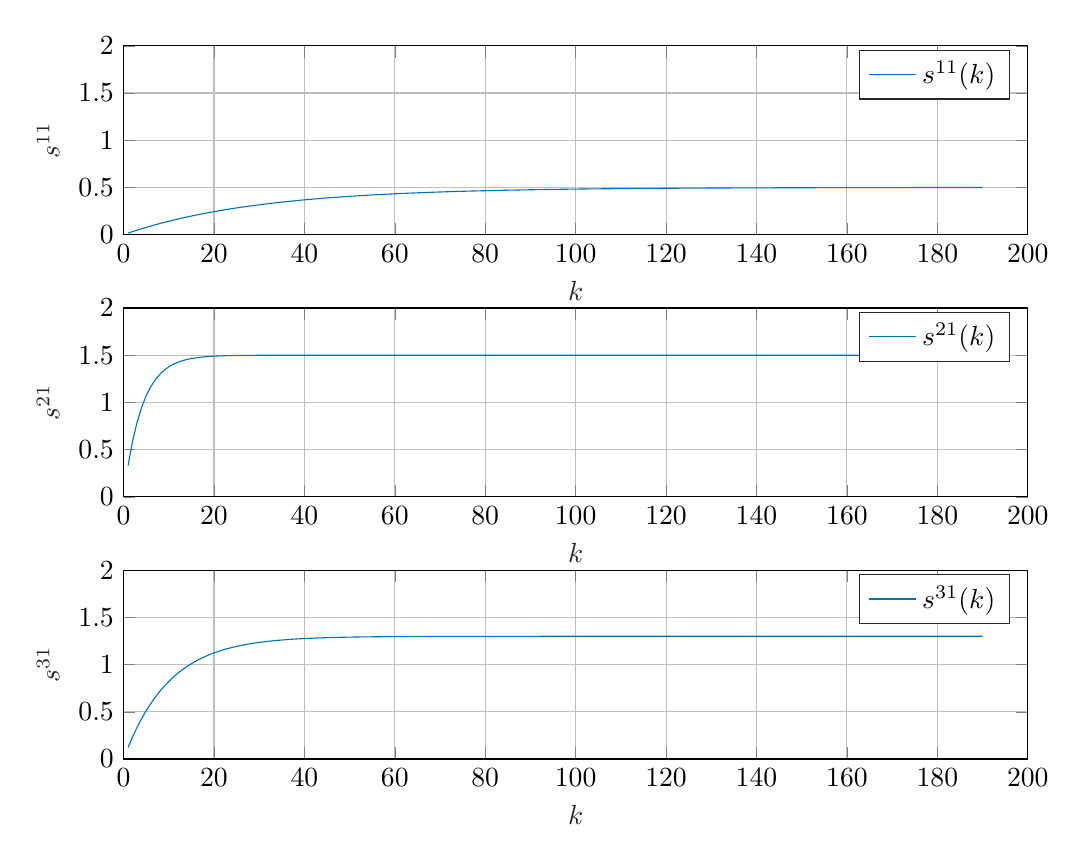
\begin{tikzpicture}

\begin{axis}[%
width=4.521in,
height=0.944in,
at={(0.758in,3.103in)},
scale only axis,
xmin=0,
xmax=200,
xlabel style={font=\color{white!15!black}},
xlabel={$k$},
ymin=0,
ymax=2,
ylabel style={font=\color{white!15!black}},
ylabel={$s^\mathrm{11}$},
axis background/.style={fill=white},
xmajorgrids,
ymajorgrids,
legend style={legend cell align=left, align=left, draw=white!15!black}
]
\addplot [color=mycolor1]
  table[row sep=crcr]{%
1	0.016391949758997\\
2	0.0322465074841911\\
3	0.0475812909820201\\
4	0.062413340478526\\
5	0.0767591375546924\\
6	0.090634623461008\\
7	0.104055216831607\\
8	0.117035830817673\\
9	0.129590889659137\\
10	0.141734344713099\\
11	0.15347968995677\\
12	0.164839976982168\\
13	0.175827829499228\\
14	0.186455457363449\\
15	0.196734670143654\\
16	0.206676890244947\\
17	0.216293165601451\\
18	0.225594181952928\\
19	0.234590274718921\\
20	0.243291440483617\\
21	0.251707348104191\\
22	0.259847349454977\\
23	0.2677204898194\\
24	0.275335517941222\\
25	0.28270089574627\\
26	0.289824807745442\\
27	0.296715170129456\\
28	0.303379639565428\\
29	0.309825621705067\\
30	0.316060279413944\\
31	0.322090540730962\\
32	0.327923106566894\\
33	0.333564458150526\\
34	0.339020864230694\\
35	0.344298388042198\\
36	0.349402894043361\\
37	0.354340054432691\\
38	0.359115355451912\\
39	0.36373410348235\\
40	0.368201430941458\\
41	0.372522301986031\\
42	0.376701518028447\\
43	0.380743723072064\\
44	0.384653408871698\\
45	0.38843491992493\\
46	0.392092458299765\\
47	0.395630088304035\\
48	0.399051741001713\\
49	0.402361218581163\\
50	0.405562198580191\\
51	0.408658237972571\\
52	0.411652777120606\\
53	0.414549143598109\\
54	0.417350555888045\\
55	0.420060126958958\\
56	0.422680867724145\\
57	0.425215690387421\\
58	0.427667411679207\\
59	0.430038755986516\\
60	0.432332358380331\\
61	0.434550767543732\\
62	0.436696448604029\\
63	0.438771785872048\\
64	0.440779085491606\\
65	0.442720578002133\\
66	0.44459842081728\\
67	0.446414700622264\\
68	0.448171435692624\\
69	0.449870578136957\\
70	0.451514016066128\\
71	0.453103575691364\\
72	0.454641023353569\\
73	0.4561280674861\\
74	0.457566360513212\\
75	0.458957500686244\\
76	0.460303033859627\\
77	0.461604455208656\\
78	0.462863210890946\\
79	0.46408069965343\\
80	0.46525827438666\\
81	0.46639724362816\\
82	0.467498873016492\\
83	0.468564386697651\\
84	0.469594968685351\\
85	0.47059176417672\\
86	0.47155588082486\\
87	0.472488389969683\\
88	0.473390327828401\\
89	0.474262696646987\\
90	0.475106465813881\\
91	0.475922572937191\\
92	0.476711924886574\\
93	0.477475398800964\\
94	0.478213843063259\\
95	0.47892807824306\\
96	0.479618898008494\\
97	0.480287070008154\\
98	0.480933336724117\\
99	0.481558416297004\\
100	0.482163003323983\\
101	0.482747769630621\\
102	0.483313365017423\\
103	0.483860417981896\\
104	0.484389536416952\\
105	0.4849013082864\\
106	0.485396302278303\\
107	0.485875068436915\\
108	0.486338138773889\\
109	0.486786027859466\\
110	0.487219233394266\\
111	0.487638236762341\\
112	0.488043503566098\\
113	0.488435484143682\\
114	0.488814614069396\\
115	0.48918131463772\\
116	0.489535993331458\\
117	0.489879044274539\\
118	0.490210848669971\\
119	0.490531775223443\\
120	0.490842180553033\\
121	0.491142409585487\\
122	0.491432795939509\\
123	0.491713662296479\\
124	0.491985320759024\\
125	0.492248073197829\\
126	0.492502211587083\\
127	0.492748018328919\\
128	0.49298576656723\\
129	0.493215720491185\\
130	0.493438135628803\\
131	0.493653259130898\\
132	0.493861330045716\\
133	0.494062579584571\\
134	0.494257231378765\\
135	0.494445501728097\\
136	0.494627599841215\\
137	0.494803728068089\\
138	0.494974082124871\\
139	0.495138851311373\\
140	0.495298218721421\\
141	0.495452361446312\\
142	0.495601450771598\\
143	0.495745652367426\\
144	0.495885126472625\\
145	0.496020028072774\\
146	0.496150507072419\\
147	0.49627670846165\\
148	0.496398772477217\\
149	0.496516834758362\\
150	0.496631026497545\\
151	0.496741474586224\\
152	0.496848301755861\\
153	0.496951626714302\\
154	0.497051564277687\\
155	0.497148225498036\\
156	0.49724171778665\\
157	0.497332145033469\\
158	0.497419607722515\\
159	0.497504203043552\\
160	0.497586025000085\\
161	0.497665164513816\\
162	0.497741709525682\\
163	0.49781574509357\\
164	0.497887353486839\\
165	0.497956614277738\\
166	0.498023604429827\\
167	0.498088398383501\\
168	0.498151068138707\\
169	0.498211683334955\\
170	0.498270311328698\\
171	0.498327017268186\\
172	0.49838186416585\\
173	0.498434912968332\\
174	0.498486222624205\\
175	0.498535850149474\\
176	0.498583850690941\\
177	0.49863027758748\\
178	0.498675182429308\\
179	0.498718615115314\\
180	0.498760623908505\\
181	0.498801255489641\\
182	0.498840555009103\\
183	0.498878566137068\\
184	0.498915331112033\\
185	0.498950890787754\\
186	0.49898528467864\\
187	0.499018551003663\\
188	0.49905072672883\\
189	0.499081847608257\\
190	0.4991119482239\\
};
\addlegendentry{$s^\mathrm{11}(k)$}

\end{axis}

\begin{axis}[%
width=4.521in,
height=0.944in,
at={(0.758in,1.792in)},
scale only axis,
xmin=0,
xmax=200,
xlabel style={font=\color{white!15!black}},
xlabel={$k$},
ymin=0,
ymax=2,
ylabel style={font=\color{white!15!black}},
ylabel={$s^\mathrm{21}$},
axis background/.style={fill=white},
xmajorgrids,
ymajorgrids,
legend style={legend cell align=left, align=left, draw=white!15!black}
]
\addplot [color=mycolor1]
  table[row sep=crcr]{%
1	0.331798825392893\\
2	0.59020401043105\\
3	0.791450170888477\\
4	0.948180838242834\\
5	1.07024280470971\\
6	1.16530475977734\\
7	1.23933908482431\\
8	1.29699707514504\\
9	1.34190116315714\\
10	1.37687250206406\\
11	1.4041082081898\\
12	1.42531939744802\\
13	1.44183868825217\\
14	1.45470392486619\\
15	1.46472338121557\\
16	1.47252654166638\\
17	1.47860364913586\\
18	1.48333650519186\\
19	1.4870224571944\\
20	1.48989307950028\\
21	1.49212872239996\\
22	1.49386984284084\\
23	1.49522582880357\\
24	1.49628187173311\\
25	1.49710431879353\\
26	1.49774484120817\\
27	1.49824368056619\\
28	1.49863217704879\\
29	1.49893473841359\\
30	1.49917037344136\\
31	1.49935388618545\\
32	1.49949680605418\\
33	1.4996081121598\\
34	1.49969479744195\\
35	1.4997623080075\\
36	1.49981488528875\\
37	1.49985583251649\\
38	1.49988772224945\\
39	1.49991255799838\\
40	1.49993190009902\\
41	1.49994696374208\\
42	1.49995869531902\\
43	1.49996783188027\\
44	1.49997494744125\\
45	1.49998048904565\\
46	1.49998480485143\\
47	1.49998816600429\\
48	1.49999078367271\\
49	1.49999282231487\\
50	1.49999441001092\\
51	1.49999564650979\\
52	1.49999660949603\\
53	1.49999735947041\\
54	1.499997943551\\
55	1.49999839843337\\
56	1.49999875269607\\
57	1.4999990285961\\
58	1.49999924346721\\
59	1.49999941080895\\
60	1.4999995411348\\
61	1.49999964263263\\
62	1.49999972167918\\
63	1.49999978324065\\
64	1.49999983118474\\
65	1.4999998685236\\
66	1.4999998976031\\
67	1.4999999202502\\
68	1.49999993788775\\
69	1.49999995162386\\
70	1.49999996232152\\
71	1.49999997065284\\
72	1.49999997714125\\
73	1.4999999821944\\
74	1.49999998612978\\
75	1.49999998919463\\
76	1.49999999158151\\
77	1.4999999934404\\
78	1.49999999488808\\
79	1.49999999601552\\
80	1.49999999689354\\
81	1.49999999757733\\
82	1.49999999810984\\
83	1.49999999852455\\
84	1.4999999988475\\
85	1.49999999909899\\
86	1.49999999929484\\
87	1.49999999944735\\
88	1.4999999995661\\
89	1.49999999965857\\
90	1.49999999973057\\
91	1.49999999978663\\
92	1.49999999983028\\
93	1.49999999986427\\
94	1.49999999989073\\
95	1.49999999991132\\
96	1.49999999992736\\
97	1.49999999993984\\
98	1.49999999994955\\
99	1.4999999999571\\
100	1.49999999996297\\
101	1.49999999996753\\
102	1.49999999997108\\
103	1.49999999997382\\
104	1.49999999997595\\
105	1.49999999997759\\
106	1.49999999997885\\
107	1.49999999997982\\
108	1.49999999998056\\
109	1.49999999998111\\
110	1.49999999998153\\
111	1.49999999998184\\
112	1.49999999998207\\
113	1.49999999998222\\
114	1.49999999998233\\
115	1.4999999999824\\
116	1.49999999998245\\
117	1.49999999998247\\
118	1.49999999998247\\
119	1.49999999998246\\
120	1.49999999998244\\
121	1.49999999998242\\
122	1.49999999998238\\
123	1.49999999998234\\
124	1.4999999999823\\
125	1.49999999998225\\
126	1.49999999998221\\
127	1.49999999998216\\
128	1.49999999998211\\
129	1.49999999998206\\
130	1.49999999998201\\
131	1.49999999998195\\
132	1.4999999999819\\
133	1.49999999998185\\
134	1.49999999998179\\
135	1.49999999998174\\
136	1.49999999998168\\
137	1.49999999998163\\
138	1.49999999998157\\
139	1.49999999998152\\
140	1.49999999998148\\
141	1.49999999998144\\
142	1.4999999999814\\
143	1.49999999998136\\
144	1.49999999998133\\
145	1.49999999998131\\
146	1.49999999998128\\
147	1.49999999998126\\
148	1.49999999998124\\
149	1.49999999998123\\
150	1.49999999998121\\
151	1.4999999999812\\
152	1.4999999999812\\
153	1.49999999998119\\
154	1.49999999998119\\
155	1.49999999998119\\
156	1.49999999998119\\
157	1.49999999998121\\
158	1.49999999998122\\
159	1.49999999998124\\
160	1.49999999998127\\
161	1.49999999998131\\
162	1.49999999998135\\
163	1.49999999998139\\
164	1.49999999998144\\
165	1.49999999998149\\
166	1.49999999998154\\
167	1.4999999999816\\
168	1.49999999998165\\
169	1.4999999999817\\
170	1.49999999998174\\
171	1.49999999998178\\
172	1.49999999998182\\
173	1.49999999998185\\
174	1.49999999998188\\
175	1.4999999999819\\
176	1.49999999998192\\
177	1.49999999998193\\
178	1.49999999998194\\
179	1.49999999998194\\
180	1.49999999998194\\
181	1.49999999998194\\
182	1.49999999998193\\
183	1.49999999998192\\
184	1.4999999999819\\
185	1.49999999998188\\
186	1.49999999998186\\
187	1.49999999998184\\
188	1.49999999998182\\
189	1.4999999999818\\
190	1.49999999998178\\
};
\addlegendentry{$s^\mathrm{21}(k)$}

\end{axis}

\begin{axis}[%
width=4.521in,
height=0.944in,
at={(0.758in,0.481in)},
scale only axis,
xmin=0,
xmax=200,
xlabel style={font=\color{white!15!black}},
xlabel={$k$},
ymin=0,
ymax=2,
ylabel style={font=\color{white!15!black}},
ylabel={$s^\mathrm{31}$},
axis background/.style={fill=white},
xmajorgrids,
ymajorgrids,
legend style={legend cell align=left, align=left, draw=white!15!black}
]
\addplot [color=mycolor1]
  table[row sep=crcr]{%
1	0.123711356553253\\
2	0.235650020998624\\
3	0.336936313113767\\
4	0.428583940153668\\
5	0.511510142373575\\
6	0.586544873077761\\
7	0.654439105071158\\
8	0.715872346647593\\
9	0.77145944233719\\
10	0.821756726477076\\
11	0.867267591192423\\
12	0.908447524514033\\
13	0.94570866905564\\
14	0.97942394687572\\
15	1.00993079180679\\
16	1.03753452660663\\
17	1.06251141873106\\
18	1.08511144531146\\
19	1.10556079501001\\
20	1.12406413179174\\
21	1.14080664327035\\
22	1.15595589412808\\
23	1.16966350315934\\
24	1.18206666072262\\
25	1.19328950178765\\
26	1.20344434831993\\
27	1.21263283343674\\
28	1.22094691858547\\
29	1.22846981392475\\
30	1.23527681111969\\
31	1.2414360368861\\
32	1.24700913482567\\
33	1.25205188237574\\
34	1.25661474904873\\
35	1.26074340154794\\
36	1.26447916081527\\
37	1.2678594155851\\
38	1.27091799658332\\
39	1.27368551511658\\
40	1.27618966944057\\
41	1.27845552197342\\
42	1.28050575012888\\
43	1.28236087327943\\
44	1.2840394581211\\
45	1.28555830449517\\
46	1.28693261352666\\
47	1.28817613976228\\
48	1.28930132883056\\
49	1.29031944200189\\
50	1.29124066889509\\
51	1.29207422945854\\
52	1.29282846624654\\
53	1.29351092791436\\
54	1.29412844476776\\
55	1.29468719712298\\
56	1.29519277716138\\
57	1.29565024489791\\
58	1.29606417882346\\
59	1.29643872172788\\
60	1.29677762216245\\
61	1.29708427195662\\
62	1.29736174016461\\
63	1.2976128037815\\
64	1.29783997553636\\
65	1.29804552904048\\
66	1.2982315215424\\
67	1.2983998145176\\
68	1.29855209229875\\
69	1.29868987893306\\
70	1.29881455343548\\
71	1.29892736359034\\
72	1.29902943843958\\
73	1.29912179958261\\
74	1.29920537140079\\
75	1.29928099030897\\
76	1.29934941312659\\
77	1.29941132465222\\
78	1.2994673445172\\
79	1.29951803338719\\
80	1.29956389857343\\
81	1.29960539911011\\
82	1.29964295034857\\
83	1.29967692811421\\
84	1.29970767246795\\
85	1.2997354911096\\
86	1.29976066245747\\
87	1.29978343843489\\
88	1.29980404699149\\
89	1.29982269438464\\
90	1.2998395672437\\
91	1.29985483443792\\
92	1.29986864876653\\
93	1.29988114848795\\
94	1.29989245870361\\
95	1.29990269260995\\
96	1.29991195263133\\
97	1.29992033144517\\
98	1.29992791290944\\
99	1.29993477290201\\
100	1.29994098007996\\
101	1.29994659656684\\
102	1.29995167857432\\
103	1.29995627696485\\
104	1.29996043776066\\
105	1.29996420260439\\
106	1.29996760917588\\
107	1.29997069156922\\
108	1.29997348063405\\
109	1.29997600428427\\
110	1.29997828777741\\
111	1.29998035396745\\
112	1.2999822235335\\
113	1.29998391518682\\
114	1.29998544585804\\
115	1.29998683086664\\
116	1.29998808407423\\
117	1.29998921802336\\
118	1.29999024406296\\
119	1.29999117246198\\
120	1.29999201251214\\
121	1.29999277262097\\
122	1.29999346039587\\
123	1.29999408272033\\
124	1.29999464582278\\
125	1.29999515533894\\
126	1.29999561636823\\
127	1.29999603352478\\
128	1.29999641098362\\
129	1.29999675252251\\
130	1.29999706155967\\
131	1.29999734118805\\
132	1.29999759420627\\
133	1.29999782314661\\
134	1.2999980303004\\
135	1.2999982177409\\
136	1.29999838734407\\
137	1.29999854080736\\
138	1.29999867966669\\
139	1.29999880531181\\
140	1.29999891900021\\
141	1.29999902186973\\
142	1.29999911494992\\
143	1.29999919917235\\
144	1.29999927537996\\
145	1.29999934433546\\
146	1.29999940672897\\
147	1.29999946318496\\
148	1.29999951426845\\
149	1.2999995604907\\
150	1.29999960231432\\
151	1.29999964015789\\
152	1.29999967440017\\
153	1.29999970538386\\
154	1.29999973341907\\
155	1.29999975878636\\
156	1.29999978173964\\
157	1.29999980250862\\
158	1.29999982130117\\
159	1.29999983830536\\
160	1.29999985369139\\
161	1.29999986761325\\
162	1.29999988021025\\
163	1.2999998916085\\
164	1.29999990192205\\
165	1.29999991125413\\
166	1.29999991969814\\
167	1.29999992733859\\
168	1.29999993425195\\
169	1.29999994050742\\
170	1.2999999461676\\
171	1.29999995128914\\
172	1.2999999559233\\
173	1.29999996011647\\
174	1.2999999639106\\
175	1.29999996734367\\
176	1.29999997045004\\
177	1.2999999732608\\
178	1.29999997580408\\
179	1.29999997810533\\
180	1.29999998018758\\
181	1.29999998207169\\
182	1.29999998377649\\
183	1.29999998531906\\
184	1.29999998671483\\
185	1.29999998797778\\
186	1.29999998912054\\
187	1.29999999015455\\
188	1.29999999109016\\
189	1.29999999193673\\
190	1.29999999270273\\
};
\addlegendentry{$s^\mathrm{31}(k)$}

\end{axis}
\end{tikzpicture}%
\caption{Odpowiedzi skokowe dla jednostkowego skoku sygna�u steruj�cego U1}
\label{odpSkok1}
\end{figure}

\begin{figure}[h!]
\centering
% This file was created by matlab2tikz.
%
\definecolor{mycolor1}{rgb}{0.00000,0.44700,0.74100}%
%
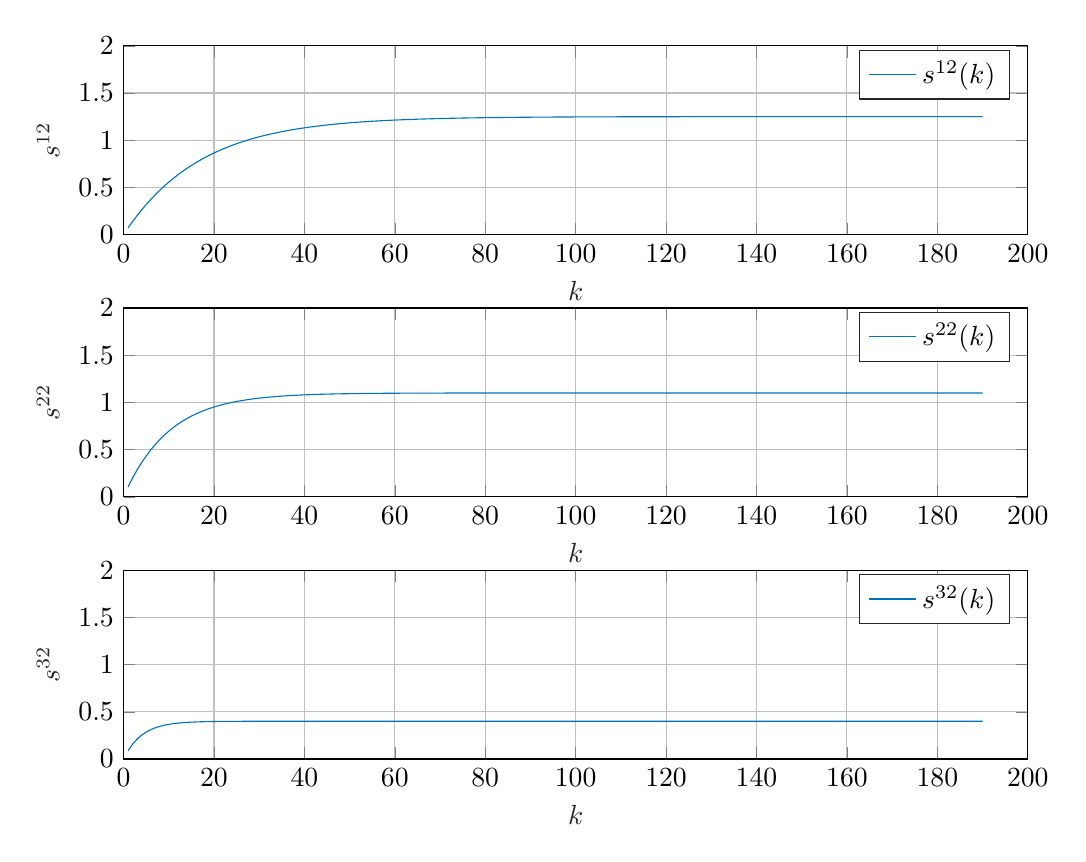
\begin{tikzpicture}

\begin{axis}[%
width=4.521in,
height=0.944in,
at={(0.758in,3.103in)},
scale only axis,
xmin=0,
xmax=200,
xlabel style={font=\color{white!15!black}},
xlabel={$k$},
ymin=0,
ymax=2,
ylabel style={font=\color{white!15!black}},
ylabel={$s^\mathrm{12}$},
axis background/.style={fill=white},
xmajorgrids,
ymajorgrids,
legend style={legend cell align=left, align=left, draw=white!15!black}
]
\addplot [color=mycolor1]
  table[row sep=crcr]{%
1	0.0714085701814063\\
2	0.13873779324653\\
3	0.20222070947125\\
4	0.262077046273127\\
5	0.318513978733148\\
6	0.371726846671253\\
7	0.421899830757587\\
8	0.469206589999648\\
9	0.513810862811794\\
10	0.55586703374754\\
11	0.595520667856222\\
12	0.632909014513543\\
13	0.668161482469864\\
14	0.701400087760479\\
15	0.732739876028188\\
16	0.762289320719905\\
17	0.790150698535544\\
18	0.816420443428697\\
19	0.841189480384364\\
20	0.864543540129004\\
21	0.8865634558622\\
22	0.90732544303697\\
23	0.926901363157113\\
24	0.945358972504636\\
25	0.962762156658172\\
26	0.979171151614094\\
27	0.994642752275675\\
28	1.00923050903192\\
29	1.02298491310646\\
30	1.03595357131807\\
31	1.04818137085763\\
32	1.0597106346519\\
33	1.07058126785194\\
34	1.08083089595294\\
35	1.09049499502387\\
36	1.0996070144974\\
37	1.10819849294526\\
38	1.11629916723974\\
39	1.12393707547912\\
40	1.13113865403326\\
41	1.1379288290453\\
42	1.14433110270623\\
43	1.15036763460071\\
44	1.15605931840604\\
45	1.16142585420939\\
46	1.1664858166939\\
47	1.17125671942945\\
48	1.17575507549074\\
49	1.17999645461241\\
50	1.18399553707914\\
51	1.18776616453708\\
52	1.19132138790264\\
53	1.19467351253442\\
54	1.19783414082458\\
55	1.20081421235708\\
56	1.20362404177182\\
57	1.20627335446579\\
58	1.2087713202546\\
59	1.21112658511113\\
60	1.21334730109101\\
61	1.21544115454856\\
62	1.21741539274084\\
63	1.2192768489119\\
64	1.22103196594405\\
65	1.22268681865798\\
66	1.22424713483897\\
67	1.22571831506194\\
68	1.22710545138394\\
69	1.22841334496881\\
70	1.229646522705\\
71	1.23080925287404\\
72	1.23190555992397\\
73	1.23293923839877\\
74	1.23391386607202\\
75	1.23483281633039\\
76	1.23569926984953\\
77	1.23651622560312\\
78	1.2372865112429\\
79	1.23801279288573\\
80	1.23869758434162\\
81	1.23934325581452\\
82	1.23995204210606\\
83	1.2405260503507\\
84	1.24106726730891\\
85	1.24157756624381\\
86	1.24205871340485\\
87	1.24251237414124\\
88	1.242940118666\\
89	1.24334342749082\\
90	1.24372369655042\\
91	1.24408224203414\\
92	1.2444203049416\\
93	1.24473905537796\\
94	1.245039596604\\
95	1.24532296885465\\
96	1.24559015293949\\
97	1.24584207363755\\
98	1.24607960289812\\
99	1.24630356285879\\
100	1.246514728691\\
101	1.24671383128308\\
102	1.24690155977002\\
103	1.24707856391869\\
104	1.24724545637681\\
105	1.24740281479349\\
106	1.24755118381852\\
107	1.2476910769876\\
108	1.24782297849972\\
109	1.24794734489313\\
110	1.24806460662547\\
111	1.2481751695637\\
112	1.24827941638885\\
113	1.24837770792062\\
114	1.24847038436619\\
115	1.24855776649778\\
116	1.24864015676291\\
117	1.24871784033121\\
118	1.24879108608148\\
119	1.24886014753231\\
120	1.24892526371957\\
121	1.24898666002376\\
122	1.24904454895012\\
123	1.24909913086411\\
124	1.24915059468494\\
125	1.24919911853949\\
126	1.24924487037878\\
127	1.24928800855932\\
128	1.24932868239124\\
129	1.249367032655\\
130	1.24940319208876\\
131	1.24943728584775\\
132	1.24946943193748\\
133	1.24949974162216\\
134	1.24952831980984\\
135	1.24955526541551\\
136	1.24958067170344\\
137	1.24960462661002\\
138	1.24962721304809\\
139	1.24964850919397\\
140	1.24966858875798\\
141	1.24968752123964\\
142	1.24970537216814\\
143	1.24972220332921\\
144	1.24973807297897\\
145	1.24975303604553\\
146	1.24976714431914\\
147	1.24978044663144\\
148	1.24979298902446\\
149	1.24980481491\\
150	1.24981596521987\\
151	1.2498264785476\\
152	1.24983639128197\\
153	1.24984573773299\\
154	1.24985455025064\\
155	1.24986285933686\\
156	1.24987069375111\\
157	1.2498780806099\\
158	1.24988504548067\\
159	1.24989161247027\\
160	1.2498978043084\\
161	1.24990364242628\\
162	1.24990914703084\\
163	1.24991433717465\\
164	1.24991923082185\\
165	1.24992384491038\\
166	1.24992819541053\\
167	1.24993229738028\\
168	1.2499361650174\\
169	1.24993981170857\\
170	1.24994325007573\\
171	1.24994649201979\\
172	1.24994954876178\\
173	1.2499524308817\\
174	1.24995514835518\\
175	1.24995771058794\\
176	1.24996012644839\\
177	1.24996240429833\\
178	1.24996455202187\\
179	1.24996657705271\\
180	1.2499684863999\\
181	1.24997028667209\\
182	1.24997198410039\\
183	1.24997358455994\\
184	1.24997509359027\\
185	1.24997651641443\\
186	1.24997785795712\\
187	1.24997912286169\\
188	1.24998031550624\\
189	1.24998144001875\\
190	1.24998250029139\\
};
\addlegendentry{$s^\mathrm{12}(k)$}

\end{axis}

\begin{axis}[%
width=4.521in,
height=0.944in,
at={(0.758in,1.792in)},
scale only axis,
xmin=0,
xmax=200,
xlabel style={font=\color{white!15!black}},
xlabel={$k$},
ymin=0,
ymax=2,
ylabel style={font=\color{white!15!black}},
ylabel={$s^\mathrm{22}$},
axis background/.style={fill=white},
xmajorgrids,
ymajorgrids,
legend style={legend cell align=left, align=left, draw=white!15!black}
]
\addplot [color=mycolor1]
  table[row sep=crcr]{%
1	0.104678840160445\\
2	0.19939617161422\\
3	0.28509995725011\\
4	0.362647949360796\\
5	0.432816274316102\\
6	0.496307200296568\\
7	0.553756165829445\\
8	0.605738139471048\\
9	0.652773374285329\\
10	0.695332614711395\\
11	0.733841807932084\\
12	0.768686366896537\\
13	0.800215027662528\\
14	0.828743339664153\\
15	0.85455682383662\\
16	0.877913830205739\\
17	0.899048123541813\\
18	0.91817122295603\\
19	0.935474518854824\\
20	0.95113118843939\\
21	0.965297928921318\\
22	0.978116525800958\\
23	0.989715271904361\\
24	1.000210251381\\
25	1.00970650151297\\
26	1.01829906396339\\
27	1.02607393598532\\
28	1.03310893111118\\
29	1.03947445793675\\
30	1.04523422479401\\
31	1.0504458773656\\
32	1.05516157562215\\
33	1.05942851585683\\
34	1.06328940304166\\
35	1.06678287823329\\
36	1.06994390530563\\
37	1.07280412088009\\
38	1.07539215095548\\
39	1.07773389740667\\
40	1.07985279721924\\
41	1.08177005705469\\
42	1.08350486549388\\
43	1.08507458508276\\
44	1.08649492610258\\
45	1.08778010380365\\
46	1.08894298067639\\
47	1.08999519518339\\
48	1.09094727824109\\
49	1.09180875861676\\
50	1.09258825829555\\
51	1.09329357877225\\
52	1.09393177913125\\
53	1.09450924669625\\
54	1.09503176095676\\
55	1.0955045514111\\
56	1.09593234990506\\
57	1.09631943798976\\
58	1.09666968977285\\
59	1.09698661069191\\
60	1.09727337259802\\
61	1.09753284550072\\
62	1.09776762629204\\
63	1.09798006473705\\
64	1.09817228699112\\
65	1.09834621687917\\
66	1.09850359514998\\
67	1.09864599689818\\
68	1.09877484732834\\
69	1.09889143601887\\
70	1.09899692982857\\
71	1.09909238457495\\
72	1.0991787556012\\
73	1.09925690733756\\
74	1.0993276219529\\
75	1.09939160718285\\
76	1.0994495034131\\
77	1.09950189008857\\
78	1.09954929151274\\
79	1.09959218209498\\
80	1.09963099109866\\
81	1.09966610693734\\
82	1.09969788106212\\
83	1.09972663147915\\
84	1.09975264593224\\
85	1.0997761847828\\
86	1.09979748361556\\
87	1.09981675559638\\
88	1.09983419360575\\
89	1.0998499721691\\
90	1.09986424920363\\
91	1.09987716759868\\
92	1.09988885664589\\
93	1.09989943333319\\
94	1.09990900351561\\
95	1.09991766297476\\
96	1.09992549837741\\
97	1.09993258814292\\
98	1.09993900322803\\
99	1.09994480783708\\
100	1.09995006006454\\
101	1.09995481247647\\
102	1.09995911263661\\
103	1.09996300358241\\
104	1.09996652425575\\
105	1.09996970989272\\
106	1.09997259237625\\
107	1.0999752005552\\
108	1.0999775605331\\
109	1.0999796959294\\
110	1.09998162811588\\
111	1.09998337643049\\
112	1.09998495837097\\
113	1.0999863897699\\
114	1.09998768495321\\
115	1.09998885688353\\
116	1.09998991728993\\
117	1.09999087678531\\
118	1.09999174497264\\
119	1.09999253054101\\
120	1.09999324135267\\
121	1.09999388452166\\
122	1.09999446648502\\
123	1.09999499306725\\
124	1.09999546953855\\
125	1.09999590066761\\
126	1.09999629076932\\
127	1.09999664374794\\
128	1.0999969631362\\
129	1.09999725213065\\
130	1.09999751362363\\
131	1.09999775023227\\
132	1.09999796432462\\
133	1.09999815804339\\
134	1.09999833332738\\
135	1.09999849193089\\
136	1.09999863544127\\
137	1.09999876529484\\
138	1.09999888279121\\
139	1.09999898910632\\
140	1.09999908530421\\
141	1.09999917234766\\
142	1.09999925110784\\
143	1.09999932237299\\
144	1.09999938685636\\
145	1.09999944520334\\
146	1.09999949799786\\
147	1.09999954576832\\
148	1.09999958899283\\
149	1.09999962810398\\
150	1.09999966349321\\
151	1.09999969551471\\
152	1.09999972448897\\
153	1.09999975070596\\
154	1.09999977442808\\
155	1.09999979589275\\
156	1.09999981531478\\
157	1.09999983288856\\
158	1.09999984878998\\
159	1.09999986317818\\
160	1.09999987619716\\
161	1.09999988797723\\
162	1.09999989863627\\
163	1.09999990828097\\
164	1.09999991700786\\
165	1.09999992490428\\
166	1.09999993204926\\
167	1.09999993851431\\
168	1.09999994436413\\
169	1.09999994965727\\
170	1.0999999544467\\
171	1.09999995878036\\
172	1.09999996270162\\
173	1.09999996624973\\
174	1.09999996946019\\
175	1.09999997236514\\
176	1.09999997499366\\
177	1.09999997737203\\
178	1.09999997952409\\
179	1.09999998147135\\
180	1.0999999832333\\
181	1.09999998482759\\
182	1.09999998627015\\
183	1.09999998757544\\
184	1.09999998875651\\
185	1.09999998982519\\
186	1.09999999079217\\
187	1.09999999166712\\
188	1.09999999245881\\
189	1.09999999317516\\
190	1.09999999382333\\
};
\addlegendentry{$s^\mathrm{22}(k)$}

\end{axis}

\begin{axis}[%
width=4.521in,
height=0.944in,
at={(0.758in,0.481in)},
scale only axis,
xmin=0,
xmax=200,
xlabel style={font=\color{white!15!black}},
xlabel={$k$},
ymin=0,
ymax=2,
ylabel style={font=\color{white!15!black}},
ylabel={$s^\mathrm{32}$},
axis background/.style={fill=white},
xmajorgrids,
ymajorgrids,
legend style={legend cell align=left, align=left, draw=white!15!black}
]
\addplot [color=mycolor1]
  table[row sep=crcr]{%
1	0.0884796867714381\\
2	0.157387736114947\\
3	0.211053378903594\\
4	0.252848223531422\\
5	0.285398081255922\\
6	0.310747935940625\\
7	0.330490422619816\\
8	0.345865886705345\\
9	0.357840310175238\\
10	0.367166000550416\\
11	0.374428855517283\\
12	0.380085172652807\\
13	0.384490316867249\\
14	0.387921046630991\\
15	0.390592901657494\\
16	0.39267374444438\\
17	0.394294306436247\\
18	0.39555640138452\\
19	0.396539321918537\\
20	0.397304821200118\\
21	0.397900992640045\\
22	0.398365291424296\\
23	0.398726887681041\\
24	0.399008499128942\\
25	0.39922781834508\\
26	0.399398624322342\\
27	0.39953164815118\\
28	0.399635247213237\\
29	0.399715930243885\\
30	0.399778766251326\\
31	0.399827702983117\\
32	0.399865814948149\\
33	0.399895496576352\\
34	0.399918612651629\\
35	0.399936615469148\\
36	0.39995063607752\\
37	0.399961555338289\\
38	0.399970059267118\\
39	0.399976682133539\\
40	0.399981840027084\\
41	0.399985856998606\\
42	0.399988985419163\\
43	0.399991421835533\\
44	0.3999933193185\\
45	0.399994797079709\\
46	0.399995947961286\\
47	0.399996844268749\\
48	0.399997542313693\\
49	0.399998085951632\\
50	0.399998509337274\\
51	0.399998839070333\\
52	0.399999095866687\\
53	0.399999295859879\\
54	0.399999451614724\\
55	0.39999957291671\\
56	0.399999667386783\\
57	0.399999740960141\\
58	0.39999979825912\\
59	0.399999842883602\\
60	0.399999877637175\\
61	0.399999904703276\\
62	0.39999992578237\\
63	0.399999942198777\\
64	0.399999954983881\\
65	0.399999964940923\\
66	0.399999972695468\\
67	0.399999978734707\\
68	0.399999983438065\\
69	0.399999987101038\\
70	0.399999989953758\\
71	0.399999992175454\\
72	0.399999993905706\\
73	0.399999995253221\\
74	0.399999996302661\\
75	0.399999997119959\\
76	0.399999997756464\\
77	0.399999998252169\\
78	0.399999998638216\\
79	0.399999998938864\\
80	0.399999999173002\\
81	0.399999999355343\\
82	0.399999999497345\\
83	0.399999999607932\\
84	0.399999999694054\\
85	0.399999999761122\\
86	0.399999999813352\\
87	0.399999999854026\\
88	0.399999999885699\\
89	0.399999999910363\\
90	0.399999999929569\\
91	0.399999999944523\\
92	0.399999999956165\\
93	0.399999999965228\\
94	0.399999999972281\\
95	0.399999999977771\\
96	0.399999999982042\\
97	0.399999999985365\\
98	0.39999999998795\\
99	0.39999999998996\\
100	0.399999999991523\\
101	0.399999999992738\\
102	0.399999999993683\\
103	0.399999999994417\\
104	0.399999999994988\\
105	0.399999999995433\\
106	0.399999999995778\\
107	0.399999999996047\\
108	0.399999999996256\\
109	0.399999999996418\\
110	0.399999999996543\\
111	0.399999999996638\\
112	0.399999999996709\\
113	0.399999999996762\\
114	0.399999999996799\\
115	0.399999999996824\\
116	0.399999999996839\\
117	0.399999999996847\\
118	0.39999999999685\\
119	0.399999999996848\\
120	0.399999999996843\\
121	0.399999999996835\\
122	0.399999999996826\\
123	0.399999999996816\\
124	0.399999999996806\\
125	0.399999999996796\\
126	0.399999999996787\\
127	0.399999999996778\\
128	0.399999999996771\\
129	0.399999999996765\\
130	0.39999999999676\\
131	0.399999999996754\\
132	0.399999999996749\\
133	0.399999999996744\\
134	0.399999999996739\\
135	0.399999999996734\\
136	0.399999999996728\\
137	0.399999999996722\\
138	0.399999999996716\\
139	0.39999999999671\\
140	0.399999999996703\\
141	0.399999999996696\\
142	0.399999999996688\\
143	0.39999999999668\\
144	0.399999999996672\\
145	0.399999999996663\\
146	0.399999999996655\\
147	0.399999999996647\\
148	0.399999999996639\\
149	0.399999999996631\\
150	0.399999999996623\\
151	0.399999999996615\\
152	0.399999999996608\\
153	0.399999999996601\\
154	0.399999999996595\\
155	0.399999999996591\\
156	0.399999999996587\\
157	0.399999999996585\\
158	0.399999999996583\\
159	0.399999999996581\\
160	0.39999999999658\\
161	0.399999999996579\\
162	0.399999999996579\\
163	0.399999999996579\\
164	0.399999999996578\\
165	0.399999999996577\\
166	0.399999999996576\\
167	0.399999999996575\\
168	0.399999999996574\\
169	0.399999999996571\\
170	0.399999999996567\\
171	0.399999999996563\\
172	0.399999999996558\\
173	0.399999999996553\\
174	0.399999999996548\\
175	0.399999999996543\\
176	0.399999999996539\\
177	0.399999999996535\\
178	0.399999999996533\\
179	0.39999999999653\\
180	0.399999999996529\\
181	0.399999999996528\\
182	0.399999999996528\\
183	0.399999999996528\\
184	0.399999999996529\\
185	0.399999999996531\\
186	0.399999999996532\\
187	0.399999999996534\\
188	0.399999999996534\\
189	0.399999999996534\\
190	0.399999999996533\\
};
\addlegendentry{$s^\mathrm{32}(k)$}

\end{axis}
\end{tikzpicture}%
\caption{Odpowiedzi skokowe dla jednostkowego skoku sygna�u steruj�cego U2}
\label{odpSkok2}
\end{figure}

\begin{figure}[h!]
\centering
% This file was created by matlab2tikz.
%
\definecolor{mycolor1}{rgb}{0.00000,0.44700,0.74100}%
%
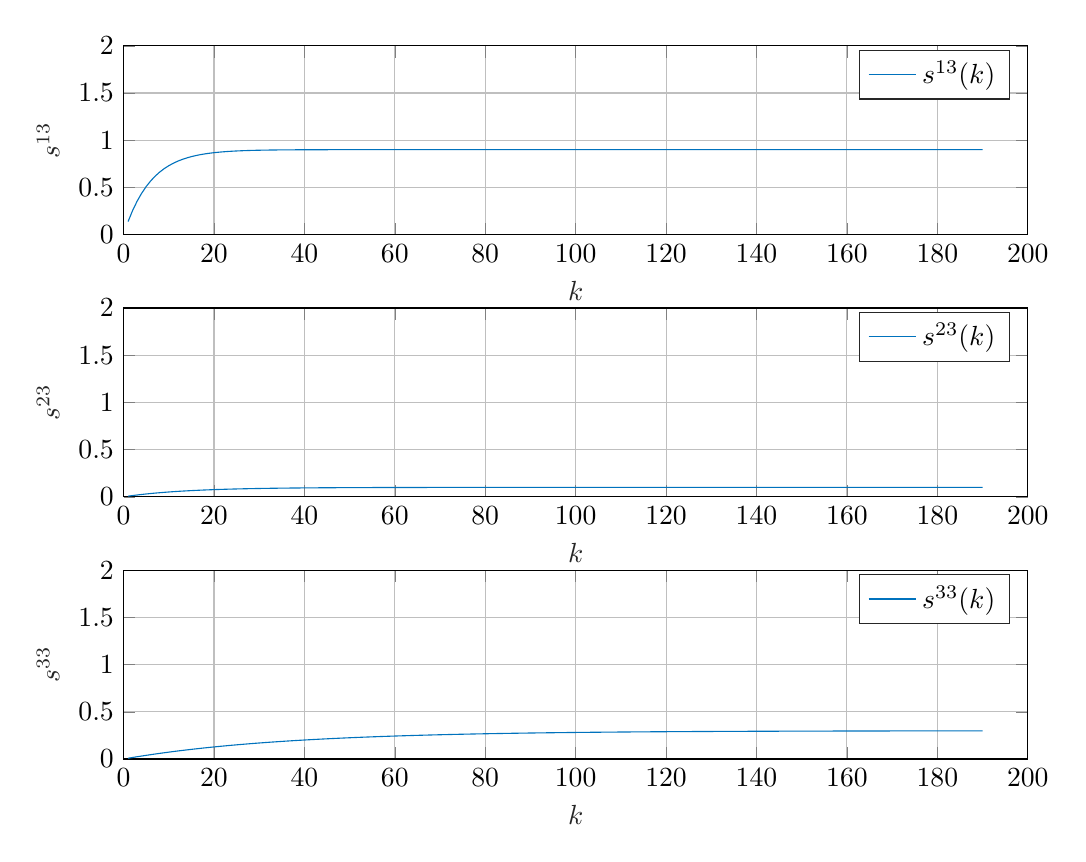
\begin{tikzpicture}

\begin{axis}[%
width=4.521in,
height=0.944in,
at={(0.758in,3.103in)},
scale only axis,
xmin=0,
xmax=200,
xlabel style={font=\color{white!15!black}},
xlabel={$k$},
ymin=0,
ymax=2,
ylabel style={font=\color{white!15!black}},
ylabel={$s^\mathrm{13}$},
axis background/.style={fill=white},
xmajorgrids,
ymajorgrids,
legend style={legend cell align=left, align=left, draw=white!15!black}
]
\addplot [color=mycolor1]
  table[row sep=crcr]{%
1	0.138166447598447\\
2	0.25512182048359\\
3	0.354122406258629\\
4	0.437924592870665\\
5	0.508861612343625\\
6	0.568908502945693\\
7	0.619737098476847\\
8	0.662762575695822\\
9	0.699182855866376\\
10	0.730011957446141\\
11	0.756108228528202\\
12	0.778198245086951\\
13	0.796897040406455\\
14	0.812725228921877\\
15	0.826123501238295\\
16	0.837464893899241\\
17	0.847065175521529\\
18	0.855191638468588\\
19	0.862070540841263\\
20	0.867893405987027\\
21	0.872822354919406\\
22	0.876994620113572\\
23	0.880526366351817\\
24	0.88351592499943\\
25	0.886046531760108\\
26	0.888188644135891\\
27	0.890001903114639\\
28	0.891536793702626\\
29	0.892836050535047\\
30	0.893935847699613\\
31	0.894866805900487\\
32	0.895654845004146\\
33	0.896321905703874\\
34	0.896886560395567\\
35	0.89736453027294\\
36	0.897769123039166\\
37	0.898111603421782\\
38	0.898401506806782\\
39	0.898646904724151\\
40	0.898854629576514\\
41	0.899030464867828\\
42	0.8991793062285\\
43	0.899305297720201\\
44	0.899411947215401\\
45	0.899502224064041\\
46	0.89957864176658\\
47	0.899643327955223\\
48	0.899698083631747\\
49	0.899744433311245\\
50	0.899783667467879\\
51	0.899816878464447\\
52	0.899844990966093\\
53	0.899868787684962\\
54	0.899888931172585\\
55	0.89990598226672\\
56	0.899920415706282\\
57	0.899932633349087\\
58	0.89994297536043\\
59	0.899951729684019\\
60	0.89995914005894\\
61	0.899965412805874\\
62	0.899970722571507\\
63	0.899975217191068\\
64	0.899979021804377\\
65	0.899982242340003\\
66	0.899984968464546\\
67	0.899987276079142\\
68	0.899989229432717\\
69	0.899990882910813\\
70	0.899992282549796\\
71	0.899993467318609\\
72	0.89999447020375\\
73	0.899995319127687\\
74	0.899996037726279\\
75	0.899996646006848\\
76	0.899997160905225\\
77	0.899997596757283\\
78	0.899997965698077\\
79	0.899998277999709\\
80	0.899998542357326\\
81	0.899998766131209\\
82	0.899998955551705\\
83	0.899999115892685\\
84	0.899999251618388\\
85	0.89999936650771\\
86	0.899999463759416\\
87	0.899999546081204\\
88	0.899999615765089\\
89	0.89999967475122\\
90	0.899999724681897\\
91	0.899999766947299\\
92	0.899999802724185\\
93	0.899999833008661\\
94	0.899999858643912\\
95	0.899999880343679\\
96	0.899999898712131\\
97	0.899999914260684\\
98	0.899999927422246\\
99	0.899999938563264\\
100	0.899999947993928\\
101	0.899999955976809\\
102	0.899999962734169\\
103	0.899999968454147\\
104	0.899999973296002\\
105	0.899999977394543\\
106	0.899999980863881\\
107	0.89999998380061\\
108	0.899999986286496\\
109	0.899999988390752\\
110	0.899999990171963\\
111	0.899999991679725\\
112	0.899999992956015\\
113	0.899999994036372\\
114	0.899999994950873\\
115	0.899999995724983\\
116	0.899999996380253\\
117	0.899999996934928\\
118	0.899999997404452\\
119	0.899999997801897\\
120	0.899999998138327\\
121	0.899999998423111\\
122	0.899999998664175\\
123	0.899999998868233\\
124	0.899999999040965\\
125	0.89999999918718\\
126	0.89999999931095\\
127	0.899999999415719\\
128	0.899999999504406\\
129	0.899999999579479\\
130	0.899999999643028\\
131	0.899999999696822\\
132	0.899999999742358\\
133	0.899999999780903\\
134	0.89999999981353\\
135	0.899999999841148\\
136	0.899999999864525\\
137	0.89999999988431\\
138	0.899999999901056\\
139	0.89999999991523\\
140	0.899999999927226\\
141	0.899999999937379\\
142	0.899999999945971\\
143	0.899999999953244\\
144	0.899999999959398\\
145	0.899999999964608\\
146	0.899999999969017\\
147	0.899999999972748\\
148	0.899999999975906\\
149	0.899999999978578\\
150	0.899999999980839\\
151	0.899999999982751\\
152	0.899999999984368\\
153	0.899999999985735\\
154	0.899999999986891\\
155	0.899999999987868\\
156	0.899999999988693\\
157	0.89999999998939\\
158	0.899999999989978\\
159	0.899999999990475\\
160	0.899999999990893\\
161	0.899999999991245\\
162	0.89999999999154\\
163	0.899999999991788\\
164	0.899999999991995\\
165	0.89999999999217\\
166	0.899999999992317\\
167	0.899999999992441\\
168	0.899999999992544\\
169	0.899999999992632\\
170	0.899999999992705\\
171	0.899999999992767\\
172	0.899999999992818\\
173	0.89999999999286\\
174	0.899999999992894\\
175	0.899999999992922\\
176	0.899999999992944\\
177	0.899999999992962\\
178	0.899999999992975\\
179	0.899999999992984\\
180	0.89999999999299\\
181	0.899999999992992\\
182	0.899999999992992\\
183	0.89999999999299\\
184	0.899999999992986\\
185	0.899999999992981\\
186	0.899999999992975\\
187	0.899999999992968\\
188	0.89999999999296\\
189	0.899999999992951\\
190	0.899999999992942\\
};
\addlegendentry{$s^\mathrm{13}(k)$}

\end{axis}

\begin{axis}[%
width=4.521in,
height=0.944in,
at={(0.758in,1.792in)},
scale only axis,
xmin=0,
xmax=200,
xlabel style={font=\color{white!15!black}},
xlabel={$k$},
ymin=0,
ymax=2,
ylabel style={font=\color{white!15!black}},
ylabel={$s^\mathrm{23}$},
axis background/.style={fill=white},
xmajorgrids,
ymajorgrids,
legend style={legend cell align=left, align=left, draw=white!15!black}
]
\addplot [color=mycolor1]
  table[row sep=crcr]{%
1	0.00689372202959773\\
2	0.0133122100249818\\
3	0.0192882252994611\\
4	0.0248522706924714\\
5	0.030032746262487\\
6	0.0348560942468945\\
7	0.0393469340287367\\
8	0.043528187799224\\
9	0.0474211975574216\\
10	0.0510458340443036\\
11	0.0544205981671963\\
12	0.0575627154323016\\
13	0.0604882238673059\\
14	0.0632120558828479\\
15	0.0657481144906843\\
16	0.0681093442675879\\
17	0.0703077974271904\\
18	0.0723546953370178\\
19	0.0742604857947106\\
20	0.0760348963557821\\
21	0.0776869839851079\\
22	0.0792251812855811\\
23	0.0806573395398914\\
24	0.0819907687851242\\
25	0.0832322751247277\\
26	0.0843881954682976\\
27	0.0854644298764967\\
28	0.0864664716762062\\
29	0.0873994354996219\\
30	0.0882680833904132\\
31	0.089076849110196\\
32	0.089829860769385\\
33	0.0905309618979376\\
34	0.0911837310635401\\
35	0.0917915001373698\\
36	0.0923573713006665\\
37	0.0928842328789185\\
38	0.0933747740844838\\
39	0.0938314987428957\\
40	0.0942567380729148\\
41	0.0946526625855609\\
42	0.0950212931628571\\
43	0.0953645113728374\\
44	0.0956840690734659\\
45	0.0959815973544879\\
46	0.096258614862856\\
47	0.0965165355542231\\
48	0.0967566759100698\\
49	0.0969802616573026\\
50	0.0971884340246227\\
51	0.0973822555675964\\
52	0.0975627155921633\\
53	0.097730735204261\\
54	0.0978871720113445\\
55	0.0980328244997949\\
56	0.0981684361105613\\
57	0.0982946990338408\\
58	0.0984122577421621\\
59	0.0985217122799092\\
60	0.0986236213260744\\
61	0.0987185050458732\\
62	0.0988068477457769\\
63	0.0988891003455151\\
64	0.0989656826796644\\
65	0.0990369856405728\\
66	0.0991033731735566\\
67	0.0991651841345534\\
68	0.0992227340197145\\
69	0.0992763165757636\\
70	0.0993262052993417\\
71	0.0993726548329916\\
72	0.0994159022649072\\
73	0.0994561683390812\\
74	0.0994936585820291\\
75	0.0995285643518395\\
76	0.0995610638149065\\
77	0.0995913228553283\\
78	0.0996194959216143\\
79	0.099645726815023\\
80	0.099670149423554\\
81	0.0996928884053402\\
82	0.0997140598249295\\
83	0.0997337717457024\\
84	0.0997521247814503\\
85	0.0997692126099296\\
86	0.0997851224510124\\
87	0.0997999355118754\\
88	0.0998137274014982\\
89	0.0998265685165875\\
90	0.0998385244008968\\
91	0.0998496560797753\\
92	0.0998600203716542\\
93	0.0998696701780604\\
94	0.099878654753636\\
95	0.0998870199575454\\
96	0.0998948084875496\\
97	0.0999020600979447\\
98	0.0999088118024759\\
99	0.099915098063264\\
100	0.0999209509667068\\
101	0.0999264003872552\\
102	0.0999314741398985\\
103	0.0999361981221378\\
104	0.0999405964461725\\
105	0.0999446915619741\\
106	0.0999485043718752\\
107	0.0999520543372598\\
108	0.0999553595778985\\
109	0.0999584369644347\\
110	0.0999613022044971\\
111	0.0999639699228738\\
112	0.0999664537361607\\
113	0.0999687663222636\\
114	0.0999709194851086\\
115	0.0999729242148919\\
116	0.0999747907441762\\
117	0.0999765286001199\\
118	0.0999781466531053\\
119	0.0999796531620153\\
120	0.0999810558163887\\
121	0.0999823617756684\\
122	0.0999835777057453\\
123	0.0999847098129824\\
124	0.0999857638758933\\
125	0.0999867452746369\\
126	0.0999876590184788\\
127	0.0999885097713599\\
128	0.0999893018757019\\
129	0.0999900393745719\\
130	0.0999907260323196\\
131	0.0999913653537905\\
132	0.099991960602216\\
133	0.0999925148158694\\
134	0.0999930308235737\\
135	0.099993511259141\\
136	0.0999939585748154\\
137	0.0999943750537903\\
138	0.099994762821862\\
139	0.0999951238582804\\
140	0.0999954600058514\\
141	0.0999957729803429\\
142	0.0999960643792427\\
143	0.099996335689912\\
144	0.0999965882971778\\
145	0.0999968234904007\\
146	0.0999970424700564\\
147	0.0999972463538632\\
148	0.099997436182487\\
149	0.099997612924853\\
150	0.0999977774830914\\
151	0.0999979306971423\\
152	0.0999980733490425\\
153	0.0999982061669173\\
154	0.0999983298286972\\
155	0.0999984449655779\\
156	0.0999985521652425\\
157	0.0999986519748605\\
158	0.0999987449038812\\
159	0.099998831426634\\
160	0.0999989119847491\\
161	0.0999989869894121\\
162	0.0999990568234624\\
163	0.0999991218433477\\
164	0.0999991823809433\\
165	0.0999992387452458\\
166	0.0999992912239505\\
167	0.0999993400849197\\
168	0.09999938557755\\
169	0.0999994279340452\\
170	0.0999994673706019\\
171	0.0999995040885126\\
172	0.099999538275193\\
173	0.0999995701051392\\
174	0.0999995997408179\\
175	0.0999996273334957\\
176	0.0999996530240114\\
177	0.0999996769434949\\
178	0.099999699214036\\
179	0.0999997199493082\\
180	0.0999997392551486\\
181	0.0999997572300983\\
182	0.099999773965905\\
183	0.0999997895479919\\
184	0.0999998040558932\\
185	0.0999998175636602\\
186	0.0999998301402394\\
187	0.0999998418498242\\
188	0.0999998527521829\\
189	0.0999998629029633\\
190	0.0999998723539771\\
};
\addlegendentry{$s^\mathrm{23}(k)$}

\end{axis}

\begin{axis}[%
width=4.521in,
height=0.944in,
at={(0.758in,0.481in)},
scale only axis,
xmin=0,
xmax=200,
xlabel style={font=\color{white!15!black}},
xlabel={$k$},
ymin=0,
ymax=2,
ylabel style={font=\color{white!15!black}},
ylabel={$s^\mathrm{33}$},
axis background/.style={fill=white},
xmajorgrids,
ymajorgrids,
legend style={legend cell align=left, align=left, draw=white!15!black}
]
\addplot [color=mycolor1]
  table[row sep=crcr]{%
1	0.0082186568650955\\
2	0.0162121593279704\\
3	0.0239866756112031\\
4	0.0315482049556892\\
5	0.038902582249983\\
6	0.0460554825328159\\
7	0.0530124253722659\\
8	0.0597787791249573\\
9	0.0663597650785779\\
10	0.0727604614809088\\
11	0.078985807458478\\
12	0.0850406068278598\\
13	0.0909295318025613\\
14	0.0966571265983577\\
15	0.102227810939857\\
16	0.107645883471\\
17	0.11291552507213\\
18	0.118040802086188\\
19	0.12302566945652\\
20	0.127873973778737\\
21	0.132589456268946\\
22	0.137175755650686\\
23	0.141636410962761\\
24	0.145974864290158\\
25	0.150194463420144\\
26	0.154298464425603\\
27	0.158290034177603\\
28	0.162172252789119\\
29	0.165948115991824\\
30	0.169620537447754\\
31	0.173192350997648\\
32	0.1766663128477\\
33	0.180045103696392\\
34	0.183331330803069\\
35	0.186527529999844\\
36	0.189636167648383\\
37	0.192659642543083\\
38	0.195600287762117\\
39	0.19846037246776\\
40	0.201242103657399\\
41	0.203947627866575\\
42	0.206579032825367\\
43	0.209138349069393\\
44	0.211627551506689\\
45	0.214048560941651\\
46	0.216403245557236\\
47	0.21869342235655\\
48	0.22092085856495\\
49	0.22308727299373\\
50	0.22519433736645\\
51	0.227243677608929\\
52	0.229236875103897\\
53	0.23117546791128\\
54	0.233060951955045\\
55	0.234894782177542\\
56	0.236678373662212\\
57	0.238413102725549\\
58	0.240100307979133\\
59	0.241741291362582\\
60	0.243337319148197\\
61	0.244889622918087\\
62	0.246399400514526\\
63	0.247867816964272\\
64	0.249296005377565\\
65	0.2506850678225\\
66	0.252036076175437\\
67	0.253350072948125\\
68	0.254628072092158\\
69	0.255871059781394\\
70	0.257079995172945\\
71	0.258255811147312\\
72	0.259399415028246\\
73	0.260511689282889\\
74	0.261593492202736\\
75	0.262645658565937\\
76	0.263669000281456\\
77	0.264664307015589\\
78	0.26563234680131\\
79	0.266573866630928\\
80	0.267489593032508\\
81	0.268380232630497\\
82	0.269246472690997\\
83	0.270088981652097\\
84	0.270908409639673\\
85	0.271705388969063\\
86	0.272480534632996\\
87	0.273234444776156\\
88	0.273967701156736\\
89	0.274680869595362\\
90	0.275374500411708\\
91	0.276049128849152\\
92	0.2767052754878\\
93	0.277343446646194\\
94	0.277964134772015\\
95	0.278567818822081\\
96	0.27915496463194\\
97	0.279726025275329\\
98	0.280281441413794\\
99	0.280821641636727\\
100	0.28134704279209\\
101	0.281858050308079\\
102	0.282355058505969\\
103	0.282838450904399\\
104	0.283308600515317\\
105	0.283765870131809\\
106	0.284210612608058\\
107	0.284643171131622\\
108	0.285063879488254\\
109	0.285473062319475\\
110	0.285871035373078\\
111	0.286258105746784\\
112	0.28663457212521\\
113	0.287000725010349\\
114	0.287356846945745\\
115	0.28770321273451\\
116	0.288040089651383\\
117	0.288367737648971\\
118	0.288686409558343\\
119	0.288996351284129\\
120	0.289297801994274\\
121	0.289590994304591\\
122	0.289876154458261\\
123	0.290153502500416\\
124	0.290423252447935\\
125	0.290685612454593\\
126	0.290940784971686\\
127	0.291188966904247\\
128	0.291430349762996\\
129	0.291665119812114\\
130	0.291893458212978\\
131	0.292115541163956\\
132	0.292331540036368\\
133	0.292541621506728\\
134	0.292745947685358\\
135	0.292944676241485\\
136	0.293137960524904\\
137	0.293325949684314\\
138	0.293508788782404\\
139	0.293686618907797\\
140	0.293859577283922\\
141	0.294027797374895\\
142	0.294191408988517\\
143	0.294350538376434\\
144	0.294505308331564\\
145	0.294655838282847\\
146	0.294802244387406\\
147	0.294944639620178\\
148	0.295083133861094\\
149	0.295217833979864\\
150	0.295348843918449\\
151	0.295476264771264\\
152	0.29560019486319\\
153	0.295720729825448\\
154	0.295837962669388\\
155	0.295951983858269\\
156	0.29606288137706\\
157	0.296170740800337\\
158	0.296275645358314\\
159	0.296377676001072\\
160	0.296476911461022\\
161	0.296573428313656\\
162	0.296667301036645\\
163	0.296758602067303\\
164	0.296847401858486\\
165	0.296933768932957\\
166	0.297017769936263\\
167	0.29709946968816\\
168	0.297178931232635\\
169	0.29725621588655\\
170	0.297331383286961\\
171	0.297404491437133\\
172	0.297475596751304\\
173	0.297544754098214\\
174	0.297612016843443\\
175	0.297677436890597\\
176	0.297741064721352\\
177	0.297802949434413\\
178	0.297863138783402\\
179	0.297921679213703\\
180	0.297978615898307\\
181	0.298033992772665\\
182	0.298087852568595\\
183	0.298140236847253\\
184	0.298191186031207\\
185	0.298240739435626\\
186	0.298288935298622\\
187	0.29833581081075\\
188	0.298381402143713\\
189	0.298425744478271\\
190	0.298468872031388\\
};
\addlegendentry{$s^\mathrm{33}(k)$}

\end{axis}
\end{tikzpicture}%
\caption{Odpowiedzi skokowe dla jednostkowego skoku sygna�u steruj�cego U3}
\label{odpSkok3}
\end{figure}

\begin{figure}[h!]
\centering
% This file was created by matlab2tikz.
%
\definecolor{mycolor1}{rgb}{0.00000,0.44700,0.74100}%
%
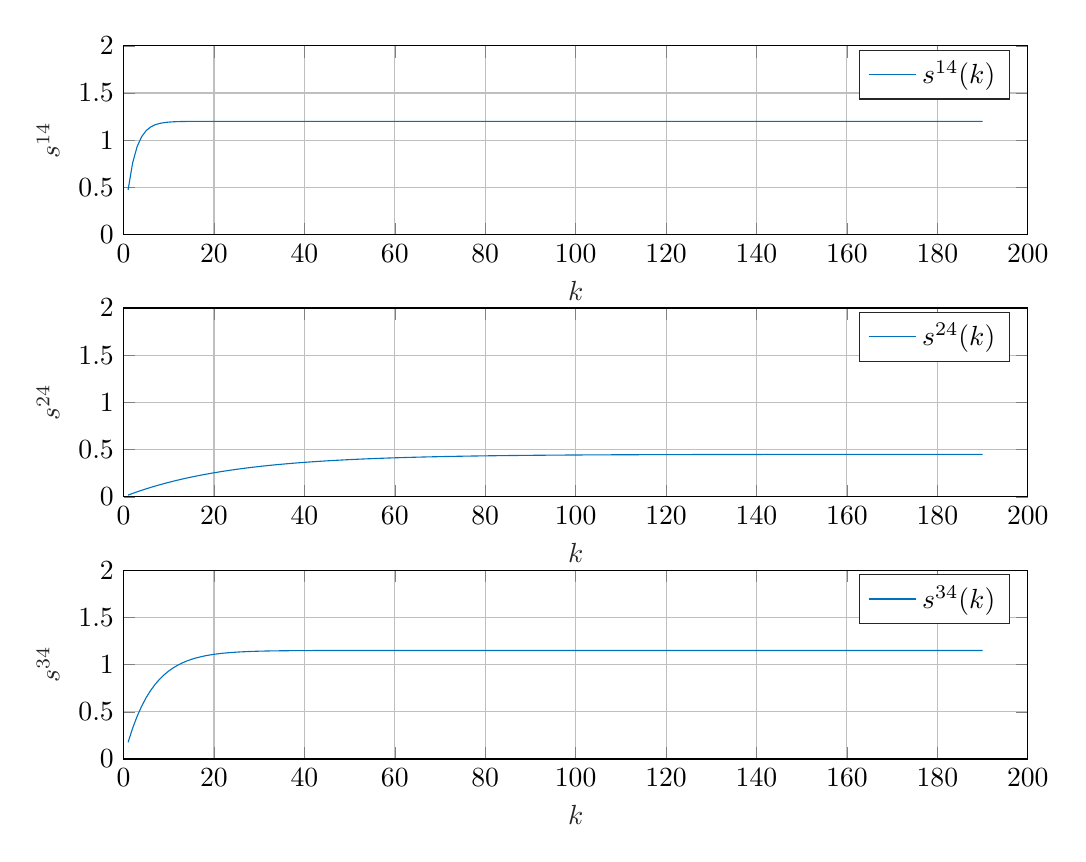
\begin{tikzpicture}

\begin{axis}[%
width=4.521in,
height=0.944in,
at={(0.758in,3.103in)},
scale only axis,
xmin=0,
xmax=200,
xlabel style={font=\color{white!15!black}},
xlabel={$k$},
ymin=0,
ymax=2,
ylabel style={font=\color{white!15!black}},
ylabel={$s^\mathrm{14}$},
axis background/.style={fill=white},
xmajorgrids,
ymajorgrids,
legend style={legend cell align=left, align=left, draw=white!15!black}
]
\addplot [color=mycolor1]
  table[row sep=crcr]{%
1	0.47216320834484\\
2	0.758544670594269\\
3	0.932243807821883\\
4	1.03759766011606\\
5	1.10149800165132\\
6	1.14025551795856\\
7	1.16376313989321\\
8	1.1780212333335\\
9	1.18666920415408\\
10	1.19191446360106\\
11	1.19509587427378\\
12	1.19702549738792\\
13	1.19819587296831\\
14	1.19890574164119\\
15	1.19933629875564\\
16	1.1995974448463\\
17	1.19975583795693\\
18	1.1998519082348\\
19	1.1999101778038\\
20	1.19994552008391\\
21	1.19996695626037\\
22	1.19997995795861\\
23	1.19998784388721\\
24	1.19999262694467\\
25	1.19999552801566\\
26	1.19999728760416\\
27	1.19999835484852\\
28	1.19999900216494\\
29	1.19999939478218\\
30	1.19999963291658\\
31	1.19999977735238\\
32	1.19999986495712\\
33	1.19999991809208\\
34	1.19999995032006\\
35	1.19999996986731\\
36	1.19999998172331\\
37	1.19999998891434\\
38	1.19999999327591\\
39	1.19999999592133\\
40	1.19999999752586\\
41	1.19999999849905\\
42	1.19999999908931\\
43	1.19999999944732\\
44	1.19999999966446\\
45	1.19999999979616\\
46	1.19999999987603\\
47	1.19999999992447\\
48	1.19999999995385\\
49	1.19999999997166\\
50	1.19999999998246\\
51	1.199999999989\\
52	1.19999999999297\\
53	1.19999999999537\\
54	1.19999999999682\\
55	1.19999999999769\\
56	1.19999999999821\\
57	1.19999999999852\\
58	1.1999999999987\\
59	1.19999999999879\\
60	1.19999999999884\\
61	1.19999999999886\\
62	1.19999999999886\\
63	1.19999999999885\\
64	1.19999999999884\\
65	1.19999999999882\\
66	1.1999999999988\\
67	1.19999999999877\\
68	1.19999999999874\\
69	1.19999999999872\\
70	1.19999999999869\\
71	1.19999999999866\\
72	1.19999999999864\\
73	1.19999999999862\\
74	1.1999999999986\\
75	1.19999999999858\\
76	1.19999999999857\\
77	1.19999999999856\\
78	1.19999999999855\\
79	1.19999999999854\\
80	1.19999999999854\\
81	1.19999999999854\\
82	1.19999999999854\\
83	1.19999999999854\\
84	1.19999999999854\\
85	1.19999999999854\\
86	1.19999999999854\\
87	1.19999999999854\\
88	1.19999999999854\\
89	1.19999999999855\\
90	1.19999999999855\\
91	1.19999999999855\\
92	1.19999999999855\\
93	1.19999999999855\\
94	1.19999999999856\\
95	1.19999999999856\\
96	1.19999999999857\\
97	1.19999999999858\\
98	1.19999999999858\\
99	1.19999999999859\\
100	1.1999999999986\\
101	1.19999999999861\\
102	1.19999999999862\\
103	1.19999999999863\\
104	1.19999999999865\\
105	1.19999999999866\\
106	1.19999999999867\\
107	1.19999999999868\\
108	1.19999999999869\\
109	1.1999999999987\\
110	1.19999999999871\\
111	1.19999999999871\\
112	1.19999999999872\\
113	1.19999999999872\\
114	1.19999999999872\\
115	1.19999999999873\\
116	1.19999999999873\\
117	1.19999999999873\\
118	1.19999999999873\\
119	1.19999999999873\\
120	1.19999999999873\\
121	1.19999999999873\\
122	1.19999999999872\\
123	1.19999999999872\\
124	1.19999999999872\\
125	1.19999999999872\\
126	1.19999999999873\\
127	1.19999999999873\\
128	1.19999999999873\\
129	1.19999999999873\\
130	1.19999999999873\\
131	1.19999999999873\\
132	1.19999999999873\\
133	1.19999999999873\\
134	1.19999999999873\\
135	1.19999999999873\\
136	1.19999999999873\\
137	1.19999999999873\\
138	1.19999999999873\\
139	1.19999999999873\\
140	1.19999999999872\\
141	1.19999999999871\\
142	1.1999999999987\\
143	1.19999999999869\\
144	1.19999999999868\\
145	1.19999999999867\\
146	1.19999999999866\\
147	1.19999999999865\\
148	1.19999999999864\\
149	1.19999999999863\\
150	1.19999999999862\\
151	1.19999999999861\\
152	1.1999999999986\\
153	1.19999999999859\\
154	1.19999999999858\\
155	1.19999999999857\\
156	1.19999999999856\\
157	1.19999999999854\\
158	1.19999999999853\\
159	1.19999999999852\\
160	1.19999999999851\\
161	1.19999999999851\\
162	1.1999999999985\\
163	1.19999999999849\\
164	1.19999999999848\\
165	1.19999999999846\\
166	1.19999999999845\\
167	1.19999999999844\\
168	1.19999999999842\\
169	1.1999999999984\\
170	1.19999999999838\\
171	1.19999999999836\\
172	1.19999999999834\\
173	1.19999999999832\\
174	1.19999999999829\\
175	1.19999999999827\\
176	1.19999999999824\\
177	1.19999999999822\\
178	1.19999999999819\\
179	1.19999999999817\\
180	1.19999999999814\\
181	1.19999999999812\\
182	1.19999999999809\\
183	1.19999999999807\\
184	1.19999999999805\\
185	1.19999999999803\\
186	1.19999999999801\\
187	1.19999999999799\\
188	1.19999999999798\\
189	1.19999999999796\\
190	1.19999999999794\\
};
\addlegendentry{$s^\mathrm{14}(k)$}

\end{axis}

\begin{axis}[%
width=4.521in,
height=0.944in,
at={(0.758in,1.792in)},
scale only axis,
xmin=0,
xmax=200,
xlabel style={font=\color{white!15!black}},
xlabel={$k$},
ymin=0,
ymax=2,
ylabel style={font=\color{white!15!black}},
ylabel={$s^\mathrm{24}$},
axis background/.style={fill=white},
xmajorgrids,
ymajorgrids,
legend style={legend cell align=left, align=left, draw=white!15!black}
]
\addplot [color=mycolor1]
  table[row sep=crcr]{%
1	0.0183647443008878\\
2	0.0359800134168046\\
3	0.0528763938369321\\
4	0.0690832237992236\\
5	0.084628644232214\\
6	0.0995396476178671\\
7	0.113842124860304\\
8	0.127560910241792\\
9	0.140719824544057\\
10	0.153341716409792\\
11	0.165448502016175\\
12	0.177061203129297\\
13	0.188199983605562\\
14	0.198884184403446\\
15	0.209132357166412\\
16	0.21896229643528\\
17	0.228391070545999\\
18	0.237435051266462\\
19	0.246109942223826\\
20	0.254430806171698\\
21	0.262412091144534\\
22	0.270067655544659\\
23	0.277410792205475\\
24	0.284454251472639\\
25	0.291210263343277\\
26	0.297690558701694\\
27	0.303906389688437\\
28	0.309868549238089\\
29	0.315587389819715\\
30	0.321072841412494\\
31	0.326334428747766\\
32	0.331381287847414\\
33	0.336222181887306\\
34	0.340865516413348\\
35	0.345319353936554\\
36	0.349591427932484\\
37	0.353689156269365\\
38	0.357619654088193\\
39	0.361389746157198\\
40	0.365005978722113\\
41	0.368474630872829\\
42	0.371801725446168\\
43	0.374993039483713\\
44	0.378054114262845\\
45	0.380990264918405\\
46	0.383806589671696\\
47	0.386507978682841\\
48	0.389099122541876\\
49	0.39158452041331\\
50	0.393968487848304\\
51	0.396255164278036\\
52	0.39844852020125\\
53	0.400552364078479\\
54	0.402570348944915\\
55	0.404505978753401\\
56	0.406362614458562\\
57	0.40814347985264\\
58	0.409851667163167\\
59	0.411490142422187\\
60	0.41306175061637\\
61	0.414569220626932\\
62	0.416015169967969\\
63	0.417402109331402\\
64	0.418732446946454\\
65	0.420008492761204\\
66	0.421232462453499\\
67	0.422406481278167\\
68	0.423532587757233\\
69	0.424612737219534\\
70	0.425648805195872\\
71	0.426642590675622\\
72	0.427595819230424\\
73	0.428510146010405\\
74	0.429387158618113\\
75	0.430228379865178\\
76	0.431035270416457\\
77	0.431809231326285\\
78	0.432551606471206\\
79	0.433263684883434\\
80	0.433946702989077\\
81	0.434601846755024\\
82	0.435230253748212\\
83	0.435833015110852\\
84	0.436411177455049\\
85	0.436965744680101\\
86	0.43749767971563\\
87	0.438007906193577\\
88	0.438497310051961\\
89	0.438966741073193\\
90	0.439417014359597\\
91	0.439848911748734\\
92	0.440263183170946\\
93	0.440660547951511\\
94	0.441041696059654\\
95	0.44140728930658\\
96	0.441757962494619\\
97	0.442094324519473\\
98	0.442416959427482\\
99	0.442726427429737\\
100	0.44302326587481\\
101	0.443307990181786\\
102	0.443581094735218\\
103	0.443843053743556\\
104	0.444094322062547\\
105	0.444335335985028\\
106	0.444566513998487\\
107	0.444788257511711\\
108	0.445000951551777\\
109	0.445204965432599\\
110	0.445400653396186\\
111	0.445588355227743\\
112	0.445768396845651\\
113	0.445941090867391\\
114	0.446106737152349\\
115	0.446265623322491\\
116	0.446418025261772\\
117	0.446564207595173\\
118	0.446704424148187\\
119	0.44683891838755\\
120	0.446967923843989\\
121	0.447091664517714\\
122	0.447210355267366\\
123	0.447324202183088\\
124	0.447433402944373\\
125	0.447538147163304\\
126	0.447638616713794\\
127	0.447734986047383\\
128	0.447827422496149\\
129	0.447916086563257\\
130	0.448001132201651\\
131	0.44808270708137\\
132	0.44816095284596\\
133	0.448236005358417\\
134	0.448307994937094\\
135	0.448377046581982\\
136	0.448443280191753\\
137	0.448506810771951\\
138	0.448567748634679\\
139	0.448626199590145\\
140	0.448682265130384\\
141	0.448736042605485\\
142	0.44878762539263\\
143	0.448837103058226\\
144	0.448884561513425\\
145	0.448930083163301\\
146	0.44897374704993\\
147	0.449015628989639\\
148	0.44905580170465\\
149	0.44909433494935\\
150	0.449131295631415\\
151	0.449166747927979\\
152	0.449200753397074\\
153	0.449233371084513\\
154	0.449264657626422\\
155	0.44929466734757\\
156	0.449323452355706\\
157	0.449351062632033\\
158	0.449377546117995\\
159	0.449402948798517\\
160	0.449427314781857\\
161	0.44945068637619\\
162	0.44947310416307\\
163	0.449494607067898\\
164	0.449515232427507\\
165	0.449535016054994\\
166	0.449553992301904\\
167	0.449572194117876\\
168	0.449589653107858\\
169	0.449606399586981\\
170	0.449622462633202\\
171	0.449637870137788\\
172	0.449652648853749\\
173	0.449666824442291\\
174	0.449680421517371\\
175	0.449693463688437\\
176	0.449705973601424\\
177	0.449717972978071\\
178	0.449729482653646\\
179	0.449740522613113\\
180	0.449751112025842\\
181	0.44976126927889\\
182	0.449771012008928\\
183	0.449780357132865\\
184	0.449789320877221\\
185	0.449797918806304\\
186	0.449806165849233\\
187	0.449814076325864\\
188	0.449821663971648\\
189	0.449828941961488\\
190	0.449835922932611\\
};
\addlegendentry{$s^\mathrm{24}(k)$}

\end{axis}

\begin{axis}[%
width=4.521in,
height=0.944in,
at={(0.758in,0.481in)},
scale only axis,
xmin=0,
xmax=200,
xlabel style={font=\color{white!15!black}},
xlabel={$k$},
ymin=0,
ymax=2,
ylabel style={font=\color{white!15!black}},
ylabel={$s^\mathrm{34}$},
axis background/.style={fill=white},
xmajorgrids,
ymajorgrids,
legend style={legend cell align=left, align=left, draw=white!15!black}
]
\addplot [color=mycolor1]
  table[row sep=crcr]{%
1	0.176546016375794\\
2	0.325988992840143\\
3	0.452489741330472\\
4	0.559570313112519\\
5	0.650212060216859\\
6	0.726938642652837\\
7	0.791886292498204\\
8	0.846863291166897\\
9	0.893400315829276\\
10	0.932793056736756\\
11	0.96613829200828\\
12	0.994364424277791\\
13	1.01825732940826\\
14	1.03848223695574\\
15	1.05560225158226\\
16	1.07009403109346\\
17	1.08236105761082\\
18	1.09274487137649\\
19	1.10153457996378\\
20	1.10897490765002\\
21	1.11527300906359\\
22	1.12060423681167\\
23	1.12511702367162\\
24	1.12893701527686\\
25	1.13217056835991\\
26	1.13490771195115\\
27	1.1372246539795\\
28	1.1391859030641\\
29	1.14084606457214\\
30	1.14225136094904\\
31	1.14344091865011\\
32	1.14444785750474\\
33	1.14530021284323\\
34	1.14602171606036\\
35	1.14663245534808\\
36	1.14714943499379\\
37	1.147587048816\\
38	1.14795748091905\\
39	1.14827104492457\\
40	1.14853647112481\\
41	1.14876114955261\\
42	1.1489513357357\\
43	1.14911232486401\\
44	1.14924859921901\\
45	1.14936395297009\\
46	1.14946159781226\\
47	1.14954425238668\\
48	1.1496142179734\\
49	1.14967344256392\\
50	1.14972357509745\\
51	1.1497660113709\\
52	1.14980193290084\\
53	1.14983233981946\\
54	1.14985807872037\\
55	1.14987986622961\\
56	1.149898308958\\
57	1.14991392039053\\
58	1.14992713518286\\
59	1.14993832126306\\
60	1.14994779007551\\
61	1.14995580525221\\
62	1.14996258995279\\
63	1.14996833307784\\
64	1.14997319452823\\
65	1.14997730965713\\
66	1.14998079303854\\
67	1.14998374165724\\
68	1.14998623760908\\
69	1.1499883503867\\
70	1.14999013881434\\
71	1.14999165268565\\
72	1.14999293415004\\
73	1.14999401888624\\
74	1.1499949370956\\
75	1.14999571434305\\
76	1.14999637226882\\
77	1.14999692919096\\
78	1.14999740061537\\
79	1.14999779966753\\
80	1.1499981374579\\
81	1.14999842339127\\
82	1.14999866542865\\
83	1.14999887030887\\
84	1.14999904373623\\
85	1.14999919053933\\
86	1.14999931480547\\
87	1.14999941999448\\
88	1.14999950903506\\
89	1.14999958440629\\
90	1.14999964820665\\
91	1.1499997022125\\
92	1.14999974792746\\
93	1.14999978662434\\
94	1.14999981938054\\
95	1.14999984710807\\
96	1.14999987057891\\
97	1.14999989044655\\
98	1.14999990726414\\
99	1.14999992149992\\
100	1.14999993355024\\
101	1.14999994375062\\
102	1.14999995238505\\
103	1.14999995969393\\
104	1.14999996588077\\
105	1.14999997111781\\
106	1.14999997555087\\
107	1.14999997930337\\
108	1.14999998247979\\
109	1.14999998516857\\
110	1.14999998744457\\
111	1.14999998937116\\
112	1.14999999100198\\
113	1.14999999238244\\
114	1.14999999355097\\
115	1.14999999454011\\
116	1.1499999953774\\
117	1.14999999608615\\
118	1.14999999668609\\
119	1.14999999719393\\
120	1.14999999762381\\
121	1.14999999798769\\
122	1.14999999829571\\
123	1.14999999855644\\
124	1.14999999877715\\
125	1.14999999896397\\
126	1.14999999912211\\
127	1.14999999925597\\
128	1.14999999936928\\
129	1.14999999946519\\
130	1.14999999954637\\
131	1.14999999961508\\
132	1.14999999967325\\
133	1.14999999972248\\
134	1.14999999976414\\
135	1.1499999997994\\
136	1.14999999982925\\
137	1.1499999998545\\
138	1.14999999987588\\
139	1.14999999989396\\
140	1.14999999990926\\
141	1.14999999992221\\
142	1.14999999993316\\
143	1.14999999994243\\
144	1.14999999995027\\
145	1.1499999999569\\
146	1.14999999996251\\
147	1.14999999996726\\
148	1.14999999997128\\
149	1.14999999997468\\
150	1.14999999997756\\
151	1.14999999998001\\
152	1.14999999998207\\
153	1.14999999998383\\
154	1.14999999998531\\
155	1.14999999998657\\
156	1.14999999998763\\
157	1.14999999998853\\
158	1.14999999998929\\
159	1.14999999998994\\
160	1.14999999999049\\
161	1.14999999999095\\
162	1.14999999999135\\
163	1.14999999999169\\
164	1.14999999999198\\
165	1.14999999999222\\
166	1.14999999999244\\
167	1.14999999999262\\
168	1.14999999999278\\
169	1.14999999999292\\
170	1.14999999999305\\
171	1.14999999999315\\
172	1.14999999999324\\
173	1.14999999999332\\
174	1.14999999999339\\
175	1.14999999999345\\
176	1.1499999999935\\
177	1.14999999999355\\
178	1.14999999999359\\
179	1.14999999999363\\
180	1.14999999999366\\
181	1.14999999999369\\
182	1.14999999999372\\
183	1.14999999999374\\
184	1.14999999999377\\
185	1.14999999999379\\
186	1.14999999999381\\
187	1.14999999999383\\
188	1.14999999999385\\
189	1.14999999999386\\
190	1.14999999999387\\
};
\addlegendentry{$s^\mathrm{34}(k)$}

\end{axis}
\end{tikzpicture}%
\caption{Odpowiedzi skokowe dla jednostkowego skoku sygna�u steruj�cego U4}
\label{odpSkok4}
\end{figure}

\section{Implementacja}

Do przeprowadzenia eksperymentu wykorzystany zosta� skrypt \verb+zad2.m+.